\documentclass{beamer}
\mode<presentation>
\usepackage{amsmath}
\usepackage{amssymb}
\usepackage{mathtools}
\usepackage{listings}
\usepackage{graphicx}
\usepackage{hyperref}
\usetheme{Boadilla}
\usecolortheme{lily}

\setbeamertemplate{footline}{
  \leavevmode%
  \hbox{%
    \begin{beamercolorbox}[wd=.9\paperwidth,ht=2.25ex,dp=1ex,left]{author in head/foot}%
      \hspace{1em} Arnav Makarand Yadnopavit
    \end{beamercolorbox}%
    \begin{beamercolorbox}[wd=.1\paperwidth,ht=2.25ex,dp=1ex,right]{author in head/foot}%
      \insertframenumber{} / \inserttotalframenumber\hspace*{2ex}
    \end{beamercolorbox}}%
}
\setbeamertemplate{navigation symbols}{}

\numberwithin{equation}{section}
\title{10.3.2.4.2: Consistency of Linear Equations}
\author{EE24BTECH11007 - Arnav Makarand Yadnopavit}
\date{\today}

\begin{document}

\begin{frame}
\titlepage
\end{frame}

\section*{Outline}
\begin{frame}
\tableofcontents
\end{frame}

\section{Question}
\begin{frame}
\frametitle{Question}
Is the following pair of linear equations consistent or inconsistent? If consistent, obtain the solution graphically.
\begin{align*}
    x - y &= 8, \\
    3x - 3y &= 16.
\end{align*}
\end{frame}

\section{Solution}
\subsection{Matrix Representation}
\begin{frame}
\frametitle{Matrix Representation}
The system can be represented in matrix form:
\begin{align*}
    A &= \begin{bmatrix} 1 & -1 \\ 3 & -3 \end{bmatrix}, \quad
    b = \begin{bmatrix} 8 \\ 16 \end{bmatrix}, \quad
    x = \begin{bmatrix} x \\ y \end{bmatrix}.
\end{align*}
\end{frame}

\subsection{LU Factorization}
\begin{frame}
\frametitle{LU Factorization Using Update Equations}
\begin{itemize}
    \item Given a matrix $ \mathbf{A} $ of size $ n \times n $, LU decomposition is performed row by row and column by column.
    \item The update equations are as follows:
\end{itemize}
\end{frame}

\begin{frame}
\frametitle{Step-by-Step Procedure}
\begin{enumerate}
    \item \textbf{Initialization:} 
    \begin{itemize}
        \item Start by initializing $ \mathbf{L} $ as the identity matrix $ \mathbf{L} = \mathbf{I} $ and $ \mathbf{U} $ as a copy of $ \mathbf{A} $.
    \end{itemize}
    \item \textbf{Iterative Update:}
    \begin{itemize}
        \item For each pivot $ k = 1, 2, \ldots, n $:
        \begin{enumerate}
            \item Compute the entries of $ \mathbf{U} $ using the first update equation.
            \item Compute the entries of $ \mathbf{L} $ using the second update equation.
        \end{enumerate}
    \end{itemize}
    \item \textbf{Result:}
    \begin{itemize}
        \item After completing the iterations, the matrix $ \mathbf{A} $ is decomposed into $ \mathbf{L} \cdot \mathbf{U} $, where $ \mathbf{L} $ is a lower triangular matrix with ones on the diagonal, and $ \mathbf{U} $ is an upper triangular matrix.
    \end{itemize}
\end{enumerate}
\end{frame}

\subsection{Update Equations}
\begin{frame}
\frametitle{Update for $ U_{k,j} $ (Entries of $ U $)}
For each column $ j \geq k $, the entries of $ U $ in the $ k $-th row are updated as:
\[
U_{k,j} = A_{k,j} - \sum_{m=1}^{k-1} L_{k,m} \cdot U_{m,j}, \quad \text{for } j \geq k.
\]
This equation computes the elements of the upper triangular matrix $ \mathbf{U} $ by eliminating the lower triangular portion of the matrix.
\end{frame}

\begin{frame}
\frametitle{Update for $ L_{i,k} $ (Entries of $ L $)}
For each row $ i > k $, the entries of $ L $ in the $ k $-th column are updated as:
\[
L_{i,k} = \frac{1}{U_{k,k}} \left( A_{i,k} - \sum_{m=1}^{k-1} L_{i,m} \cdot U_{m,k} \right), \quad \text{for } i > k.
\]
This equation computes the elements of the lower triangular matrix $ \mathbf{L} $, where each entry in the column is determined by the values in the rows above it.
\end{frame}

\subsection{LU Decomposition Result}
\begin{frame}
\frametitle{LU Decomposition Result}
Using code, we compute:
\[
L = \begin{bmatrix} 1 & 0 \\ 3 & 1 \end{bmatrix}, \quad
U = \begin{bmatrix} 1 & -1 \\ 0 & 0 \end{bmatrix}.
\]
\end{frame}

\subsection{Solving $A x = b$}
\begin{frame}
\frametitle{Solving $A x = b$}
\textbf{Forward Substitution: Solve $L y = b$}
\begin{align*}
    \begin{bmatrix} 1 & 0 \\ 3 & 1 \end{bmatrix} \begin{bmatrix} y_1 \\ y_2 \end{bmatrix} = \begin{bmatrix} 8 \\ 16 \end{bmatrix}.
\end{align*}
\begin{itemize}
    \item $y_1 = 8$.
    \item $3y_1 + y_2 = 16 \implies y_2 = -8$.
\end{itemize}
\end{frame}

\begin{frame}
\frametitle{Back Substitution: Solve $U x = y$}
\begin{align*}
    \begin{bmatrix} 1 & -1 \\ 0 & 0 \end{bmatrix} \begin{bmatrix} x \\ y \end{bmatrix} = \begin{bmatrix} 8 \\ -8 \end{bmatrix}.
\end{align*}
\begin{itemize}
    \item First row: $x - y = 8$.
    \item Second row: $0 = -8$ (contradiction).
\end{itemize}
\textbf{Conclusion:} The system is inconsistent.
\end{frame}

\section{Graphical Representation}
\begin{frame}
\frametitle{Graphical Representation}
\begin{figure}[h]
    \centering
    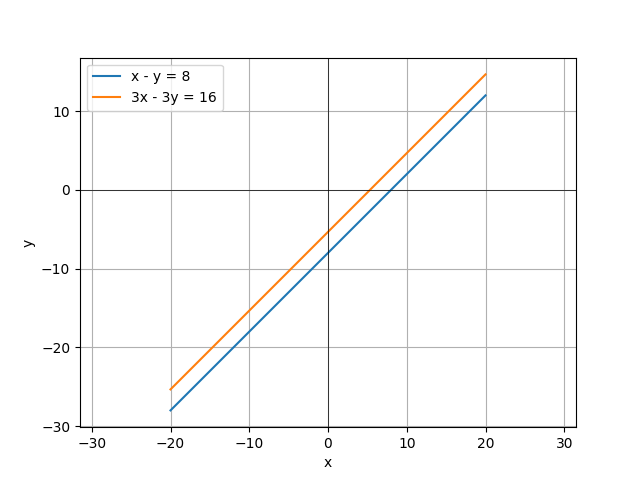
\includegraphics[width=0.8\linewidth]{figs/fig.png}
\end{figure}
\end{frame}

\end{document}

